%----------------------------------------------------------------------------------------
%	PACKAGES AND THEMES
%----------------------------------------------------------------------------------------
\documentclass[aspectratio=169,xcolor=dvipsnames, t]{beamer}
\usepackage{fontspec} % Allows using custom font. MUST be before loading the theme!
\usetheme{SimplePlusAIC}
\usepackage{hyperref}
\usepackage{graphicx} % Allows including images
\usepackage{booktabs} % Allows the use of \toprule, \midrule and  \bottomrule in tables
\usepackage{svg} %allows using svg figures
\usepackage{tikz}
\usepackage{makecell}
\usepackage{wrapfig}
\usepackage{comment}
\usepackage{animate}
\usepackage{xcolor}

\usetikzlibrary{overlay-beamer-styles}
\usetikzlibrary{shapes, positioning, calc}
\usetikzlibrary{decorations.text}
\usetikzlibrary{shapes.geometric, arrows}
% ADD YOUR PACKAGES BELOW

%----------------------------------------------------------------------------------------
%	TITLE PAGE CONFIGURATION
%----------------------------------------------------------------------------------------

\title[Section 2.3]{2.3 Scheduling jobs on identical parallel machines} % The short title appears at the bottom of every slide, the full title is only on the title page
\subtitle{CSE462: Algorithm Engineering Sessional}

\author[Samee]{Abdus Samee}
\institute[CSE462]{1805021 \newline Computer Science \& Engineering\newline Bangladesh University of Engineering  \& Technology}
% Your institution as it will appear on the bottom of every slide, maybe shorthand to save space


\date{\today} % Date, can be changed to a custom date
%----------------------------------------------------------------------------------------
%	PRESENTATION SLIDES
%----------------------------------------------------------------------------------------

\begin{document}

\maketitlepage

\begin{frame}[t]{Overview}
    % Throughout your presentation, if you choose to use \section{} and \subsection{} commands, these will automatically be printed on this slide as an overview of your presentation
    \tableofcontents
\end{frame}

%------------------------------------------------
% Section divider frame
\makesection{Introduction}

%------------------------------------------------
% Problem Definition
\begin{frame}{Problem Definition}
    \begin{itemize}
        \item \textit{m} identical machines running in parallel \pause
        \begin{itemize}
            \item Each machine can process at most $1$ job at a time \pause
        \end{itemize}
        \item \textit{n} jobs \pause
        \begin{itemize}
            \item Every job $j=1,...,n$ must be processed in one of the machines for $p_j$ time units without interruption \pause
            \item Each job is available for processing at time $0$ \pause
            \item A job $j$ completes at time $C_j$
        \end{itemize}
    \end{itemize}
\end{frame}

%------------------------------------------------
% Problem Goal
\begin{frame}{Problem Goal}
    Our goal is to complete all jobs as soon as possible \pause
    \begin{equation*}
        \text{minimize } C_{max} = max_{j=1,...,n}C_j
    \end{equation*}
    Also known as \alert{\textit{makespan}} or \alert{\textit{length}} of the schedule \pause
    \newline \newline
    Moreover, the load-balancing problem can be a similar to this, where $n$ items(or jobs) each with weight $p_j$ are distributed among $m$, in order to minimize maximum total weight assigned to one machine
\end{frame}

%------------------------------------------------
% Computational Hardness
\begin{frame}{Computational Hardness}
    \begin{itemize}
        \item The problem is NP-hard even when there are only $2$ machines \pause
        \item When $m \le 3$, then there exists a pseudo-polynomial time algorithm \pause
        \item In contrast, when $m \ge 4$, the problem is strongly NP-hard
    \end{itemize}
\end{frame}

%------------------------------------------------
% Section divider frame
\makesection{Algorithm}

%------------------------------------------------
% Local Search
\begin{frame}{Local Search}
    \onslide<1>
    \begin{block}{What is Local Search?}
        A heuristic method which moves from one feasible solution to another optimizing a criterion defined by a set of local changes
    \end{block} \pause

    \onslide<2->
    \begin{description}
        \item[Initiation] Start with a random schedule \pause
        \item[Local move] Choose the job $j$ that finishes last \pause
        \item[Base case] Find if any machine exists to which job $j$ can be reassigned \pause
        \item[Recur or End] If a machine $m$ remains free after processing its assigned jobs before $j$ starts being processed, then we assign $j$ to $m$ and continue. Otherwise, we terminate the process
    \end{description}
\end{frame}

%------------------------------------------------
% Local Search Illustration
\begin{frame}{Local Search Illustration}
    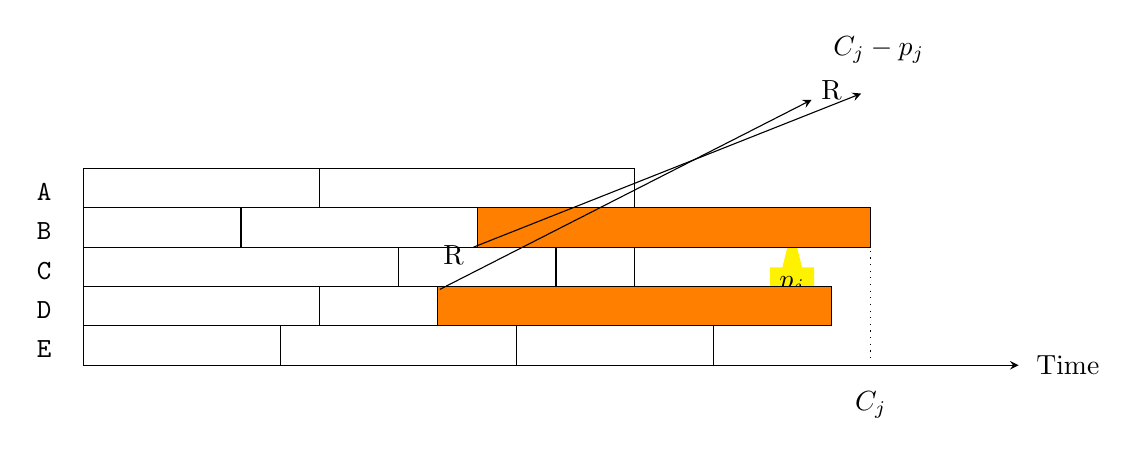
\begin{tikzpicture}
        \node (A) at (1.5,5.7) {\texttt{A}};
        \node (A) at (1.5,5.2) {\texttt{B}};
        \node (A) at (1.5,4.7) {\texttt{C}};
        \node (A) at (1.5,4.2) {\texttt{D}};
        \node (A) at (1.5,3.7) {\texttt{E}};
        
        \draw (2,5.5) rectangle (5,6);
        \draw (5,5.5) rectangle (9,6);
        \draw (2,5) rectangle (4,5.5);
        \draw (4,5) rectangle (7,5.5);
        \draw (2,4.5) rectangle (6,5);
        \draw (6,4.5) rectangle (8,5);
        \draw (8,4.5) rectangle (9,5);
        \draw (2,4) rectangle (5, 4.5);
        \draw(5,4) rectangle (6.5,4.5);
        \draw(2,3.5) rectangle (4.5,4);
        \draw(4.5,3.5) rectangle (7.5,4);
        \draw(7.5,3.5) rectangle (10,4);

        \node (a) at (7.5,3.5) {};
        \node (b) at (14,3.5) {};
        \node (c) at (14.5,3.5) {Time};
        \onslide<2> \node (d) at (12,3.4) {};
        \onslide<2> \node (dd) at (12,3) {$C_j$};
        \node (e) at (12,5.5) {};
        \onslide<2> \node (f) at (11,5.5) {};
        
        \onslide<1-> \draw[-stealth] (a) -- (b);
        \onslide<2> \draw[dotted] (e) -- (d);
        \onslide<2> \node[rectangle callout, color=black, fill=yellow, callout relative pointer={(0,0.5)}, below of=f] {$p_j$};
        \onslide<1-3> \draw [fill=orange] (7,5) rectangle (12,5.5);

        \onslide<3> \node (g) at (6.7,4.9) {R};
        \node (h) at (12,7) {};
        \onslide<3> \node (i) at (12.1,7.5) {$C_j-p_j$};
        \onslide<3> \draw[-stealth] (g) -- (h);

        \onslide<4-5> \draw [fill=orange] (6.5,4) rectangle (11.5,4.5);
        \node (j) at (6.4,4.4) {};
        \onslide<5>
        \node (k) at (11.5,7) {R};
        \draw[-stealth] (j) -- (k);
    \end{tikzpicture}
\end{frame}

\begin{frame}{Greedy Algorithm}
    \begin{itemize}
        \item Often called list scheduling algorithm \pause
        \item Assign a job as soon as a machine is available for processing \pause
        \item Pick the least heavily loaded machine $\rightarrow$ greedy choice \pause
        \item A 2-approximation algorithm of the original problem
    \end{itemize}
\end{frame}

%------------------------------------------------
% Section divider frame
\makesection{Theorem}

%------------------------------------------------
% Theoerm
\begin{frame}{Theorem}
    \begin{theorem}[2-approximation algorithm]
        The local search procedure for scheduling jobs on identical parallel machines is a 2-approximation algorithm
    \end{theorem}
\end{frame}

\begin{frame}{Proof - First Lower Bound}
    Suppose, \\
    The length of optimal schedule be $C_{max}^*$ \newline \newline \pause
    $x_{ij}=1$ if $i$ machine processes job $j$, otherwise $x_{ij}=0$ \newline \newline \pause
    For any machine $i$, its completion time is $\sum_{j=1}^{n} x_{ij}p_j$ \newline \newline \pause
    So,
    \begin{equation}\label{E1}
        C_{max}^* \ge \sum_{j=1}^{n} x_{ij}p_j
    \end{equation}
\end{frame}

\begin{frame}{Proof - Second Lower Bound}
    Moreover, \\
    The total processing time is $P=\sum_{j=1}^n p_j$ \newline \newline \pause
    $\therefore$ A machine is assigned $\frac{P}{m}$ units of work on average \newline \newline \pause
    Consequently, one machine must be assigned at least the \textbf{average} amount of work.
    So,
    \begin{equation}\label{E2}
        C_{max}^* \ge \sum_{j=1}^{n} \frac{p_j}{m} = \frac{P}{m}
    \end{equation}
\end{frame}

\begin{frame}{Proof - Illustration Revisit}
    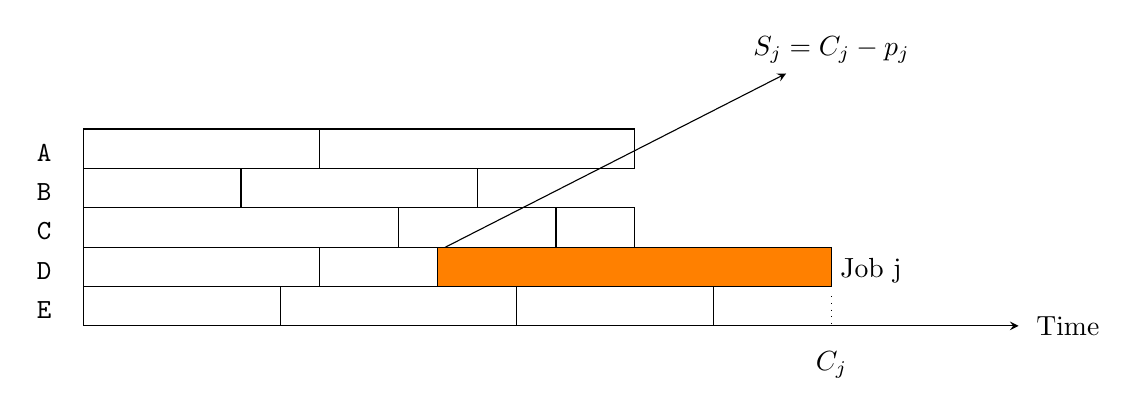
\begin{tikzpicture}
        \node (A) at (1.5,5.7) {\texttt{A}};
        \node (A) at (1.5,5.2) {\texttt{B}};
        \node (A) at (1.5,4.7) {\texttt{C}};
        \node (A) at (1.5,4.2) {\texttt{D}};
        \node (A) at (1.5,3.7) {\texttt{E}};
        
        \draw (2,5.5) rectangle (5,6);
        \draw (5,5.5) rectangle (9,6);
        \draw (2,5) rectangle (4,5.5);
        \draw (4,5) rectangle (7,5.5);
        \draw (2,4.5) rectangle (6,5);
        \draw (6,4.5) rectangle (8,5);
        \draw (8,4.5) rectangle (9,5);
        \draw (2,4) rectangle (5, 4.5);
        \draw(5,4) rectangle (6.5,4.5);
        \draw(2,3.5) rectangle (4.5,4);
        \draw(4.5,3.5) rectangle (7.5,4);
        \draw(7.5,3.5) rectangle (10,4);

        \node (a) at (7.5,3.5) {};
        \node (b) at (14,3.5) {};
        \node (c) at (14.5,3.5) {Time};
        \node (j) at (6.4,4.4) {};
        \node (k) at (11.5,7) {$S_j = C_j-p_j$};
        \node (l) at (12,4.2) {Job j};
        \node (M) at (11.5,4) {};
        \node (N) at (11.5,3.4) {};
        \node (O) at (11.5, 3) {$C_j$};
        
        \draw[-stealth] (j) -- (k);
        \draw[-stealth] (a) -- (b);
        \draw [fill=orange] (6.5,4) rectangle (11.5,4.5);
        \draw[dotted] (M) -- (N);
    \end{tikzpicture}
\end{frame}

\begin{frame}{Proof - Rounding Up}
    \onslide<1->
    Partition the schedule into time intervals $[0, S_j]$ and time during which $j$ is processed\newline \newline
    \onslide<2->
    By \eqref{E1}, length of latter interval is at most $C_{max}^*$ time\newline \newline
    \onslide<3->
    The total work processed during the first interval is $mS_j$
    \onslide<4->
    \begin{equation}\label{E3}
        S_j \le \sum_{j=1}^{n} \frac{p_j}{m}
    \end{equation}
    \onslide<5>
    From \eqref{E2} and \eqref{E3}, $S_j \le C_{max}^*$. So both intervals have a size of at most $C_{max}^*$. \textbf{Thus, the makespan of the schedule is at most $\mathbf{C_{max}^*}$.}
\end{frame}

\begin{frame}{Proof - Refinement}
        Eqn \eqref{E3} takes into account the last completed job $j$, so excluding that \newline \newline \pause
        $$p_j = \sum_{k \ne j}  \frac{p_k}{m}=(1-\frac{1}{m})p_k+\sum_{l=1}^n \frac{p_k}{m}$$ \pause
        Applying the lower bounds, we have the length of the schedule as $$(2-\frac{1}{m})C_{max}^*$$
\end{frame}

% Final PAGE
% Set the text that is shown on the final slide
\finalpagetext{Thank you for your attention}
%----------------------------------------------------------------------------------------
\makefinalpage
%----------------------------------------------------------------------------------------
\end{document}
